\documentclass[a4paper,12pt]{article}
\usepackage{graphicx}
\usepackage{titlesec}
\usepackage[utf8]{inputenc}
\usepackage{xcolor}
\usepackage{fancyhdr}
\usepackage{lipsum}
\usepackage{caption}
\usepackage{floatrow}
\usepackage{lmodern}


\renewcommand{\headrulewidth}{0pt}
\fancyhead[C]{}
\fancyhead[C]{
	
\includegraphics[width=4cm]{metu}
}
\pagestyle{plain}

%opening
\title{Middle East Technical University\\Department of Physics\\\textbf{PHYS307 Applied Modern Physics}}
\author{Oğuzhan ÖZCAN\\}
\date{}
\clearpage
\thispagestyle{empty}
\providecommand{\groupmember}[1]{\textbf{Group Members:} }
\providecommand{\expdate}[1]{\textbf{Experiment Date:} }
\providecommand{\repdate}[1]{\textbf{Report Submit Date:} }
\providecommand{\expname}[1]{\textbf{Exp. MP-ZE Zeeman Effect} }


\usepackage[a4paper,%
left=0.5in,right=0.5in,top=0.5in,bottom=0.8in,%
footskip=.25in]{geometry}
%\topmargin -4.5cm
%\oddsidemargin 0.2cm
%\textwidth 16cm %
%\textheight 21cm%
%\footskip 1.0cm%




\begin{document}
\pagenumbering{gobble}
\maketitle

\thispagestyle{fancy}

%%%%%%%%%%%%%%%%%%%%%%%%%%%%%%%%%%%%%%%%%%%%%%%%%%%%%
\noindent\rule{18.4cm}{0.8pt}
\begin{center}
	\expname{arg1}{}
\end{center}

\expdate{November 6, 2015}{December 11, 2015}\\
\repdate{arg1}{December 18, 2015}\\
\noindent\rule{18.4cm}{0.8pt}\\\\
%%%%%%%%%%%%%%%%%%%%%%%%%%%%%%%%%%%%%%%%%%%%%%%%%%%%%
\begin{table}[h!]
\begin{center}
	\begin{tabular}{|c|c|c|c|c|}
	\hline \textbf{Magnetic Current $I$ [A]}  &\textbf{ Magnetic Field Strength $B$ [T]} & 2$\delta$a & $\delta$a & $\delta a / \Delta a$ \\ 
	\hline 18 & 0.494 & 0.175 & 0.0875 & 0.486 \\ 
	\hline 16 & 0.445 & 0.14 & 0.07 & 0.388 \\ 
	\hline 14 & 0.421 & 0.13 & 0.065 & 0.361 \\ 
	\hline 12 & 0.336 & 0.115 & 0.0575 & 0.319 \\ 
	\hline 10 & 0.279 & 0.10 & 0.05 & 0.277 \\ 
	\hline 8 & 0.223 & 0.08 & 0.04 & 0.222 \\ 
	\hline 
\end{tabular} 
\end{center}
\caption{Splitting of a spectral line under various magnetic field strengths($\Delta a=0.18$ mm)}
\end{table}

\begin{figure}[h!]
	\centering
	\includegraphics[scale = 0.65]{"untitled"}
	\caption{$\delta a / \Delta a$ versus Magnetic Field Strength}
	\label{fig:untitled}
\end{figure}
 \textbf{	\textbullet The slope of the best line = 0.85 T$^{-1}$}
\newpage
\begin{figure}[h!]
	\centering
	\includegraphics[scale = 1.0]{"slope"}
	\caption{Calculation of slope by using Appendix II}
	\label{fig:slope}
\end{figure}

We can calculate slope by following calculations if $m=b \pm \Delta b$ where $b$ is correspond to $\frac{e}{m}$ and $\Delta b$ is correspond to $\Delta \frac{e}{m}$
\begin{equation}
b=\frac{\sum xy - \frac{\sum x \sum y}{n}}{\sum x^{2} - \frac{(\sum x )^{2}}{n}}
\end{equation}
\begin{equation}
b=\frac{0.7987 - \frac{(2.198)\cdot(2.053)}{6}}{0.8598 - \frac{(0.0002)^{2}}{6}}
\end{equation}
\begin{equation}
b=\frac{0.04661}{0.05459}
\end{equation}
\begin{center}
	\framebox[100pt]{$\frac{e}{m}$=b=0.853(7)}
\end{center}
\begin{equation}
\Delta b = \sqrt{\frac{\frac{1}{n-2}\sum (y-\hat{y})^{2}}{\sum (x-\bar{x})^{2}}}
\end{equation}
\begin{equation}
\Delta b = \sqrt{\frac{\frac{1}{4}\times 0.0002}{0.0546}}
\end{equation}
\begin{center}
	\framebox[100pt]{$\Delta \frac{e}{m}$=$\Delta b =0.03$}
\end{center}
Therefore, slope of $\delta a /\Delta a$ versus magnetic field strength graph is
\begin{center}
	\framebox[100pt]{m=0.853 $\pm$ 0.03}
\end{center}
\textbf{1. What is the most important general statement you can make after performing this experiment?}\\\\
When a magnetic field is applied to atoms, some of the atomic
energy levels may be changed and some levels which had identical
energies may be split into levels with different energies.In this experiment we measured the energy level splitting and
polarizations due to the Zeeman Effect.\\\\
\textbf{2. What do you think the spectral lines may correspond to?}\\\\
Spectral lines are correspond to the splitting of energy levels due to external magnetic field. This effect was a part of the classic theory of electron which is predicted by H. A. Lorentz in 1895 and experimentally confirmed by P. Zeeman.
\newpage
\textbf{3. In the measurement of the splitting, you measured $2\delta a $ instead of $\delta a $. Does this make any sense? Why?}\\\\
\begin{figure}[h!]
	\centering
	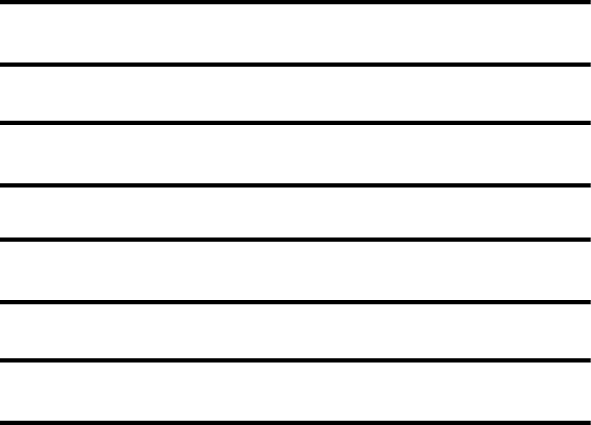
\includegraphics[scale = 0.8]{b0}
	\caption{Spectral lines when $B=0$}
	\label{fig:b0}
\end{figure}

\begin{figure}[!h]
	\begin{floatrow}
	
		\ffigbox{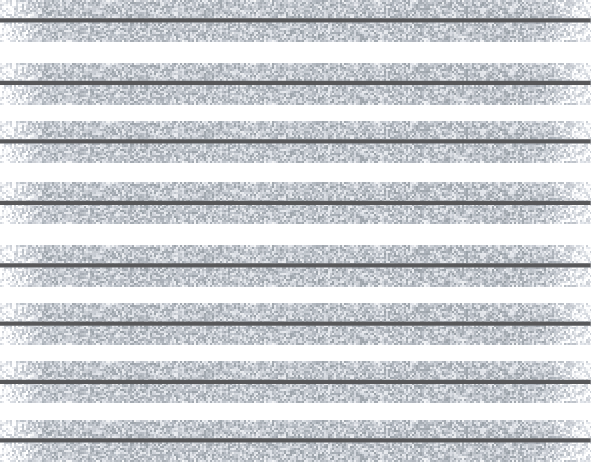
\includegraphics[scale = 0.8]{b1}}{\caption{Observed spectral lines when $B\neq 0$}\label{fig:b1}}
		\ffigbox{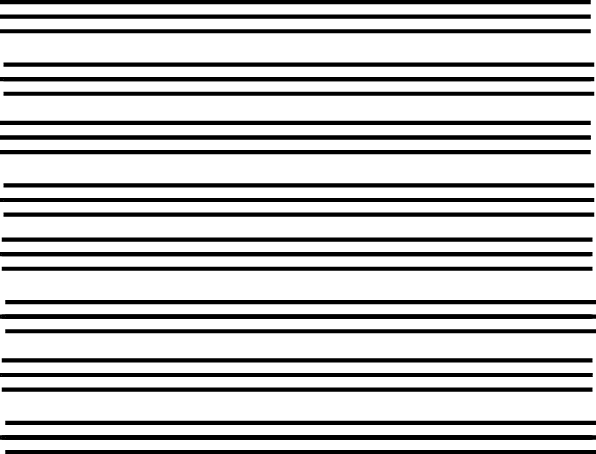
\includegraphics[scale = 0.8]{b2}}{\caption{Expected spectral lines when $B\neq 0$}\label{fig:b2}}
	\end{floatrow}
\end{figure}
According to theory, when the Zeeman effect is viewed in a direction perpendicular to the direction of the magnetic field $B$, a triplet is observed. The lines of this triplet should be sharp lines as seen Figure 5. However, in the experiment these lines are not sharp, in fact, these line are blurred or distorded as seen in Figure 4. In this case, we could not be sure about the edges of the lines. That is why, we calculated $2\delta a$ instead of $\delta a$ to have more accurate data. In Figure 6, we can see the measured splitting.\\\\
\begin{figure}[h!]
 	\centering
 	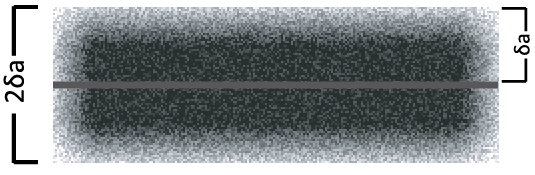
\includegraphics[scale = 1.0]{b3}
 	\caption{Close view of a spectral line}
 	\label{fig:b3}
 \end{figure}
 
\textbf{Discussion and Conclusion}\\\\
In this experiment we carried out crucial topic in Physics which is Zeeman Effect. The splitting of energy levels of an atom when it is placed in an external magnetic field is known as Zeeman Effect. P. Zeeman discovered this effect in 1896. There are two types of this effect: Normal Zeeman Effect and Anomalaus Zeeman Effect. As we mentioned above, in the experiment we could not observe three sharp lines. Even with a high resolution spectrometer the magnetic field splits spectral lines in to more than three lines. This is called as Anomalaus Zeeman Effect and it was not discovered for a long time. This effect observed in the experiment. According to our results, when magnetic field strenth increses $\delta a /\Delta a$ ratio also increases (See Figure 1). In this experiment we only observed plane polarised effect. There is also circularly polarised effect. To sum up, according to our results, this experiment is accomplished. 











































































































































\end{document}
